% ========================================================================
% ========================================================================



\section*{Installation}
\href{https://auto.gluon.ai/stable/index.html}{AutoGluon} (\href{https://github.com/awslabs/autogluon/}{GitHub}) requires pip > 1.4 (upgrade by pip install -U pip). \href{https://auto.gluon.ai/stable/index.html#installation}{More installation options}. AutoGluon supports Python 3.9 to 3.12. Installation is available for Linux, MacOS, and Windows.

\begin{minted}[fontsize=\footnotesize, bgcolor=codeback, frame=leftline, framesep=10pt]{bash}
pip install autogluon
\end{minted}

Import Autogluon Multimodal:

\begin{minted}[fontsize=\footnotesize, bgcolor=codeback, frame=leftline, framesep=10pt]{python}
from autogluon.multimodal import MultiModalPredictor
\end{minted}

\begin{center}
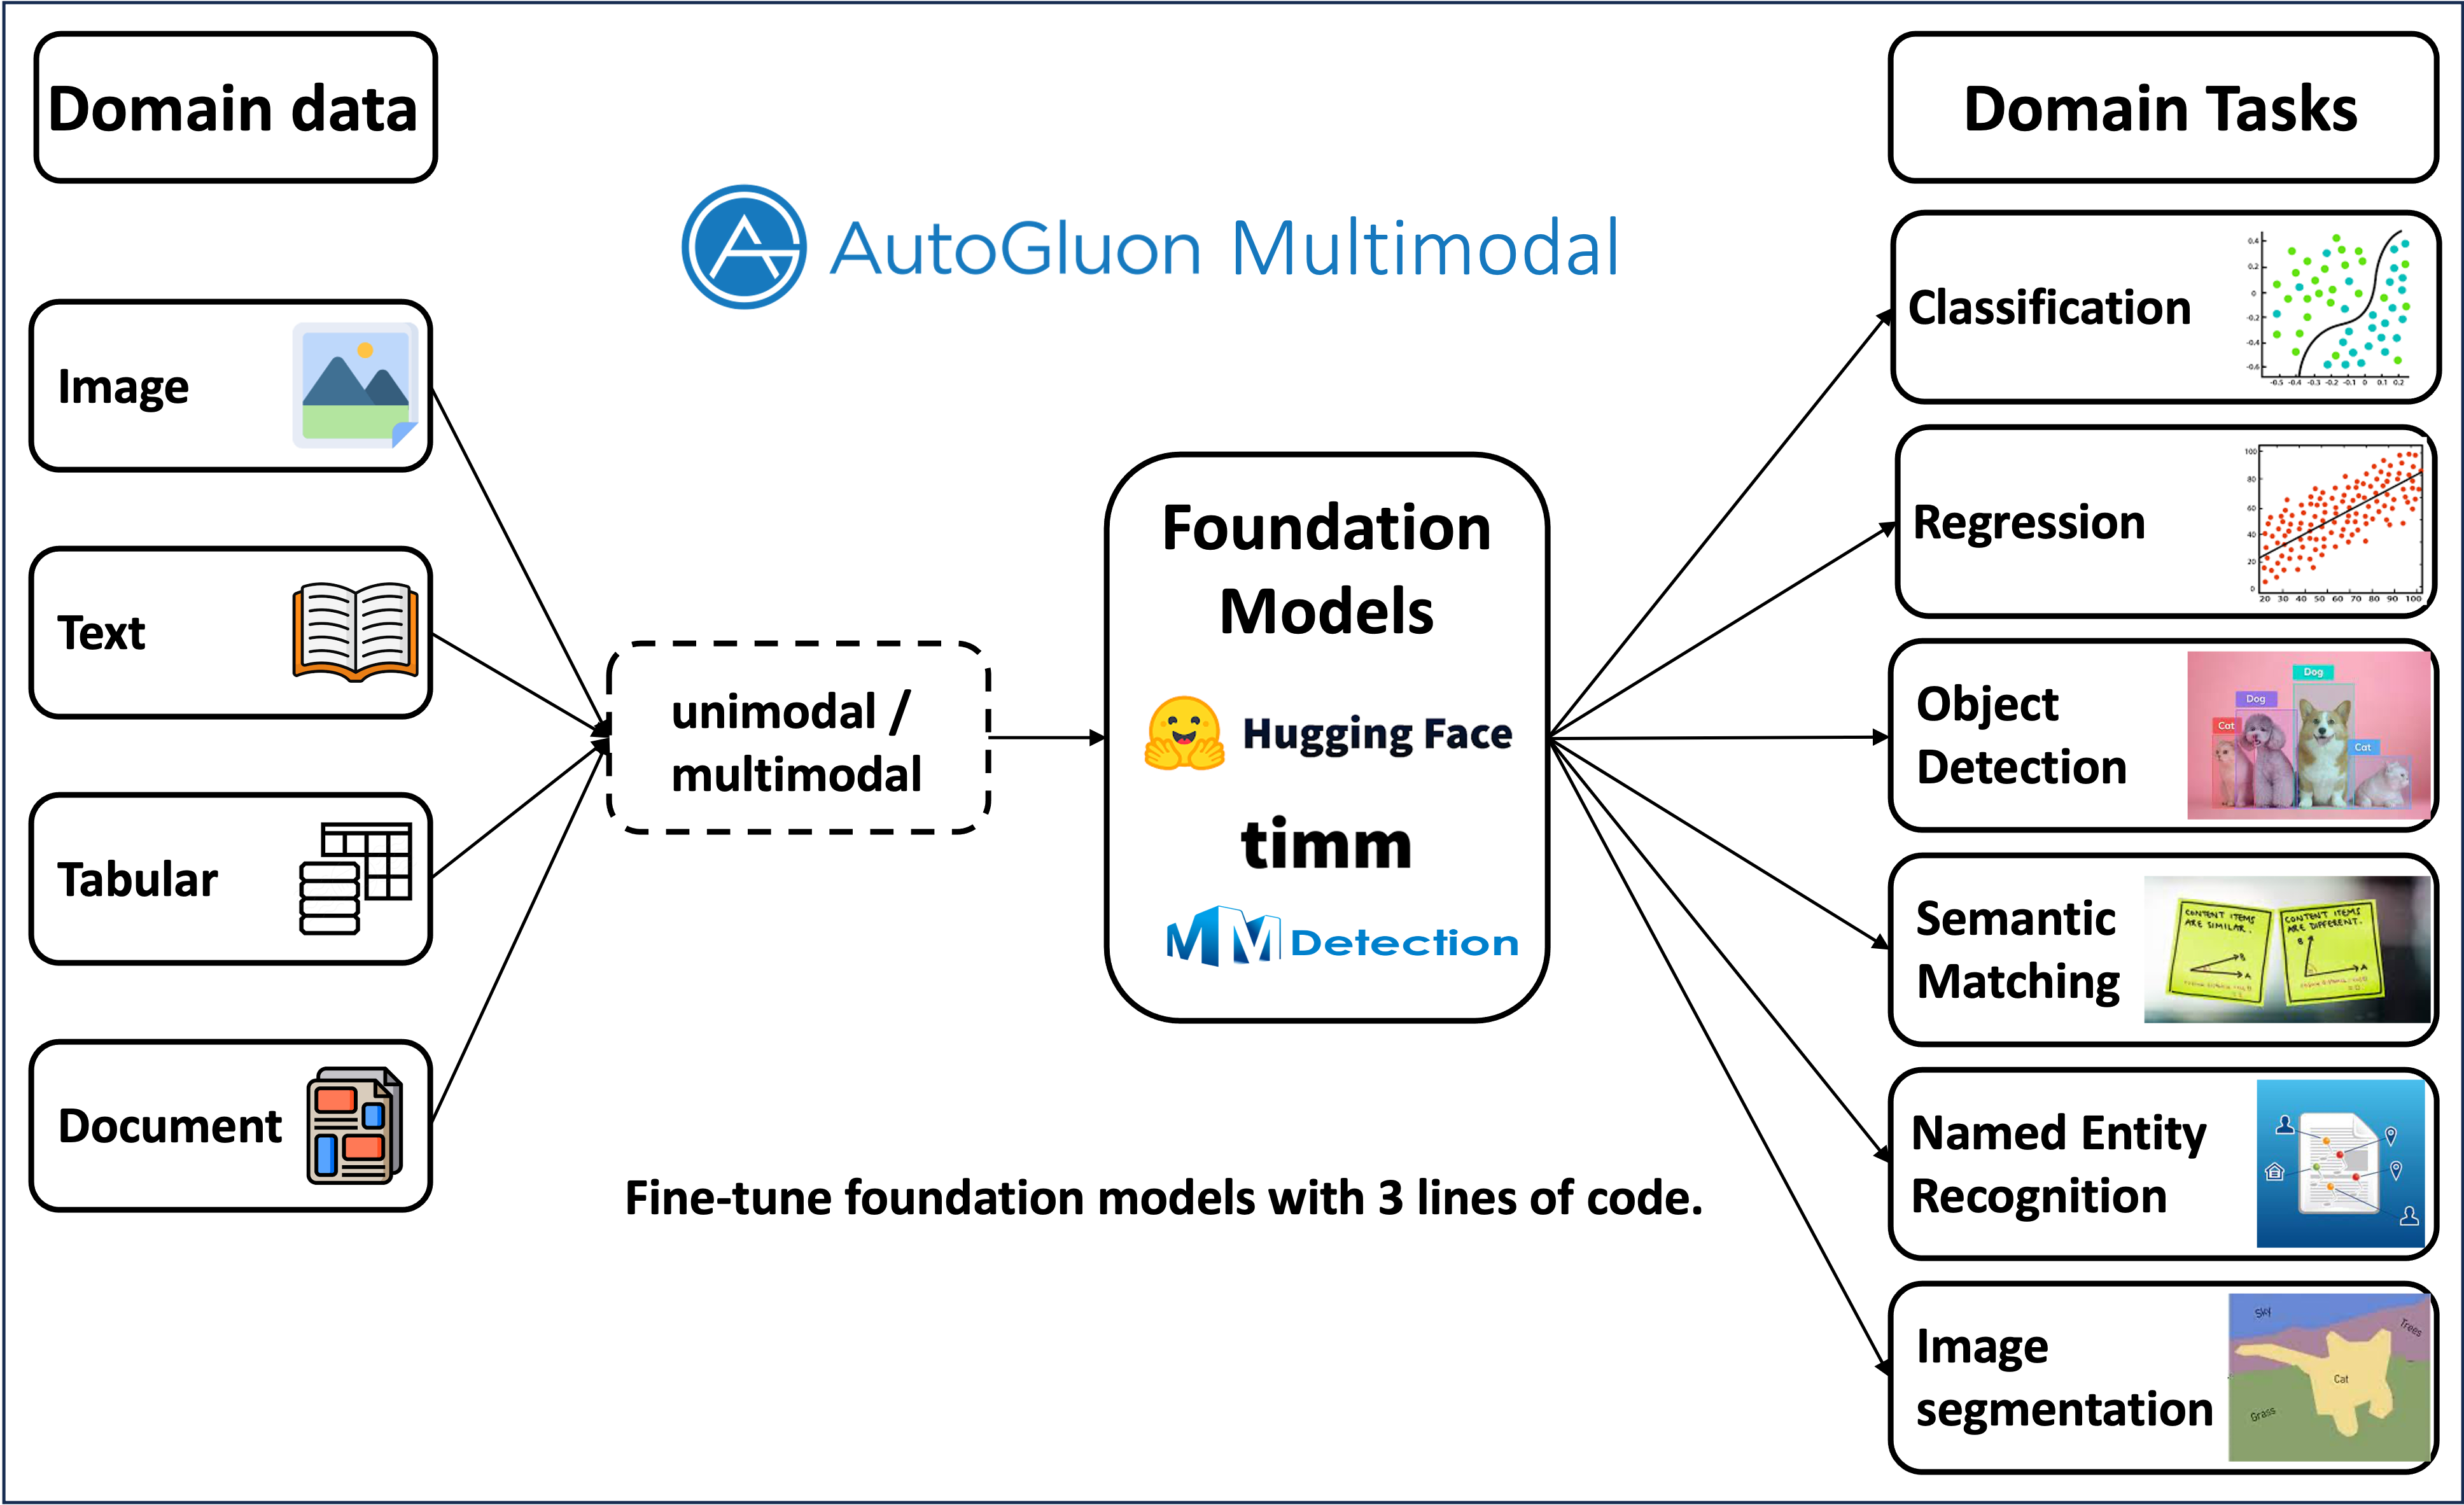
\includegraphics[width=1.0\linewidth]{images/automm-intro.png}
\end{center}

% ========================================================================

\section*{Classification \& Regression}
MultiModalPredictor finetunes foundation models for solving classification and regression problems with image, text, and tabular features. Here, we use a simplified version \href{https://automl-mm-bench.s3.amazonaws.com/petfinder_for_tutorial.zip}{petfinder\_for\_tutorial} from the \href{https://www.kaggle.com/c/petfinder-adoption-prediction}{PetFinder dataset}. MultiModalPredictor automatically analyzes the columns in the input dataframe to detect categorical, numerical, text, and images (stored as paths or bytearrays).
\begin{minted}[fontsize=\footnotesize, bgcolor=codeback, frame=leftline, framesep=10pt]{python}
import pandas as pd
train_data = pd.read_csv('train.csv', index_col=0)
test_data = pd.read_csv('test.csv', index_col=0)
\end{minted}

To train the model, just call `.fit()'. We also support customization (\href{https://auto.gluon.ai/stable/tutorials/multimodal/advanced_topics/customization.html}{docs}).

\begin{minted}[fontsize=\footnotesize, bgcolor=codeback, frame=leftline, framesep=10pt]{python}
predictor = MultiModalPredictor(
    problem_type="classification", 
    label="AdoptionSpeed"
)
predictor.fit(train_data)
\end{minted}

To extract embedding, or evaluate/inference on the test set.

\begin{minted}[fontsize=\footnotesize, bgcolor=codeback, frame=leftline, framesep=10pt]{python}
predictor.extract_embedding(test_data)
predictor.evaluate(test_data)  # Evaluation
predictor.predict(test_data)  # Inference
# To Predict probability
predictor.predict_proba(test_data)
\end{minted}


\section*{Object Detection}
To use MultiModalPredictor for object detection, please first install additional dependencies by
\begin{minted}[fontsize=\footnotesize, bgcolor=codeback, frame=leftline, framesep=10pt]{bash}
mim install "mmcv==2.1.0"
pip install "mmdet==3.2.0"
pip install "mmengine>=0.10.6"
\end{minted}

MultiModalPredictor supports common object detection data formats such as \href{https://cocodataset.org/}{COCO} (recommended) and
\href{http://host.robots.ox.ac.uk/pascal/VOC/}{VOC}. Here we use the dataset \href{https://automl-mm-bench.s3.amazonaws.com/object_detection_dataset/tiny_motorbike_coco.zip}{tiny$\_$motorbike\_coco} to demonstrate how to use MultiModalPredictor. The predictor natively supports json files in the COCO-format.
We can also \href{https://auto.gluon.ai/stable/tutorials/multimodal/object_detection/quick_start/quick_start_coco.html}{visualize the detected bounding boxes with its confidence scores}, 

\begin{minted}[fontsize=\footnotesize, bgcolor=codeback, frame=leftline, framesep=10pt]{python}
train_path = "./Annotations/trainval_cocoformat.json"
test_path = "./Annotations/test_cocoformat.json"
predictor = MultiModalPredictor(
    problem_type="object_detection",
    sample_data_path=train_path,
)
predictor.fit(train_path) # Train the detector
predictor.evaluate(test_path) # Evaluation
predictor.predict(test_path) # Inference
\end{minted}


\section*{Named-Entity Recognition}
MultiModalPredictor supports named-entity recognition. We use \href{https://groups.csail.mit.edu/sls/downloads/movie/}{MIT movies corpus} to demonstrate the usage, which can be downloaded from \href{https://automl-mm-bench.s3.amazonaws.com/ner/mit-movies/train.csv}{train.csv} and \href{https://automl-mm-bench.s3.amazonaws.com/ner/mit-movies/test.csv}{test.csv}.

\begin{minted}[fontsize=\footnotesize, bgcolor=codeback, frame=leftline, framesep=10pt]{python}
import pandas as pd
predictor = MultiModalPredictor(
    problem_type="ner", label="entity_annotations"
)
# Train model
predictor.fit(pd.read_csv("train.csv"))
# Evaluation
predictor.evaluate(pd.read_csv("test.csv"))
# Inference
text = "Game of Thrones is an American fantasy "
        "drama TV series created by David Benioff" 
pred = predictor.predict('text_snippet': [text]})
\end{minted}

\section*{Image Segmentation}
While Segment Anything Model (SAM) performs exceptionally well on generic scenes, it encounters challenges when applied to specialized domains like manufacturing, agriculture, etc. 
MultiModalPredictor mitigates the issue by fine-tuning on domain specific data. Below is an example on \href{https://www.kaggle.com/datasets/sovitrath/leaf-disease-segmentation-with-trainvalid-split}{Leaf Disease Segmentation} dataset.

\begin{minted}[fontsize=\footnotesize, bgcolor=codeback, frame=leftline, framesep=10pt]{python}
import pandas as pd
train_data = pd.read_csv('train.csv', index_col=0)
test_data = pd.read_csv('test.csv', index_col=0)
image_col, label_col = 'image', 'label'
predictor = MultiModalPredictor(
    problem_type="semantic_segmentation", 
    label=label_col,
)
# Finetuning (optional, zero-shot is also supported)
predictor.fit(train_data=train_data)
\end{minted}

Under the hood, we use LoRA for efficient fine-tuning. Note that, without hyperparameter customization, the huge SAM serves as the default model, which requires efficient fine-tuning in many cases. After fine-tuning, evaluate/predict on the test data.

\begin{minted}[fontsize=\footnotesize, bgcolor=codeback, frame=leftline, framesep=10pt]{python}
predictor.evaluate(test_data, metrics=["iou"])
pred = predictor.predict(test_data)
\end{minted}

We can visualize the image, the predicted mask before and after fine-tuning (\href{https://auto.gluon.ai/stable/tutorials/multimodal/image_segmentation/beginner_semantic_seg.html}{docs}).

\begin{center}
    \begin{minipage}{0.3\linewidth}
    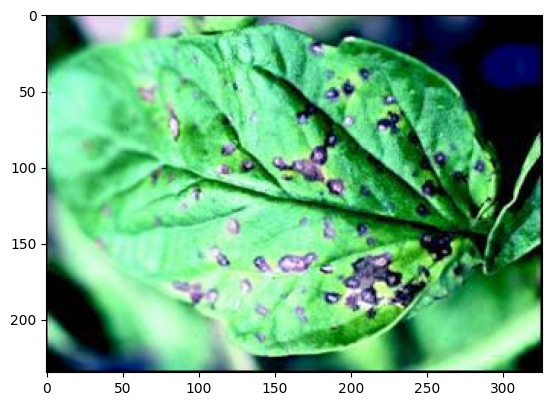
\includegraphics[width=\linewidth]{images/leaf.png}
    \center{\caption{image}}
    \end{minipage}%
    \begin{minipage}{0.3\linewidth}
    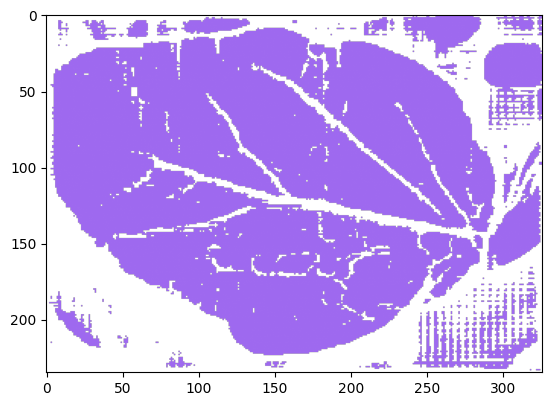
\includegraphics[width=\linewidth]{images/leaf_0seg.png}
    \center{\caption{SAM}}
    \end{minipage}%
    \begin{minipage}{0.3\linewidth}
    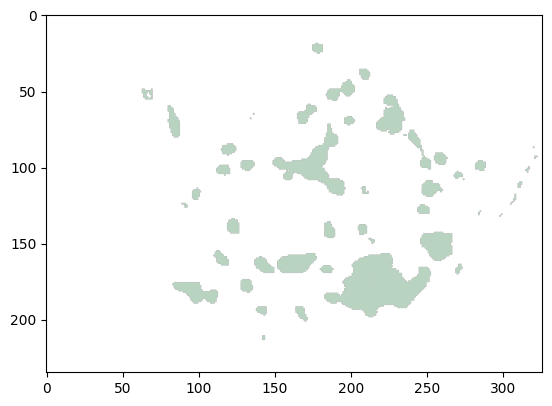
\includegraphics[width=\linewidth]{images/leaf_seg.png}
    \center{\caption{SAM+PEFT}}
    \end{minipage}%
\end{center}

As evident from the results, the predicted mask after finetuning is much closer to the groundtruth. This demonstrates the effectiveness of using MultiModalPredictor to fine-tune SAM for domain-specific applications, enhancing its performance in tasks like leaf disease segmentation

\section*{Semantic Matching}
MultiModalPredictor implements a flexible twin-tower architecture that can solve text-text, image-image, and text-image matching problems (\href{https://auto.gluon.ai/stable/tutorials/multimodal/matching/index.html}{docs}). Here is an example of finetuning the matching model via relevance data, demonstrated via the \href{https://paperswithcode.com/dataset/flickr30k}{Flickr30K} image-text matching dataset preprocessed in the dataframe format: \href{https://automl-mm-bench.s3.amazonaws.com/flickr30k.zip}{flickr30k.zip}.
\begin{minted}[fontsize=\footnotesize, bgcolor=codeback, frame=leftline, framesep=10pt]{python}
import pandas as pd
train_data = pd.read_csv("train.csv", index_col=0)
tdata = pd.read_csv("test.csv", index_col=0)
\end{minted}

To finetune model, just specify the ``query" and ``response'' keys when creating predictor and pick ``image\_text\_similarity'' as problem type.
\begin{minted}[fontsize=\footnotesize, bgcolor=codeback, frame=leftline, framesep=10pt]{python}
predictor = MultiModalPredictor(
            query="caption",
            response="image",
            problem_type="image_text_similarity",
        )
# Finetuning (optional, zero-shot is also supported)
predictor.fit(train_data, time_limit=180)
# Extract embedding
e_i = predictor.extract_embedding(tdata["image"])
e_t = predictor.extract_embedding(tdata["caption"])
\end{minted}

\begin{itemize}
  \item MultiModalPredictor also supports model and hyperparameter customization (\href{https://auto.gluon.ai/stable/tutorials/multimodal/advanced_topics/customization.html}{docs}), knowledge distillation (\href{https://auto.gluon.ai/stable/tutorials/multimodal/advanced_topics/model_distillation.html}{docs}), few shot learning (\href{https://auto.gluon.ai/stable/tutorials/multimodal/advanced_topics/few_shot_learning.html}{docs}), parameter-efficient finetuning (\href{https://auto.gluon.ai/stable/tutorials/multimodal/advanced_topics/efficient_finetuning_basic.html}{docs}), HPO (\href{https://auto.gluon.ai/stable/tutorials/multimodal/advanced_topics/hyperparameter_optimization.html}{docs}), and \href{https://auto.gluon.ai/stable/tutorials/multimodal/index.html}{more}.
  \item For deployment, check \href{https://auto.gluon.ai/stable/tutorials/cloud_fit_deploy/index.html}{AutoGluon-Cloud}.
  \item For other use-cases, check
  \href{https://auto.gluon.ai/stable/tutorials/tabular_prediction/index.html}{TabularPredictor} and
  \href{https://auto.gluon.ai/stable/tutorials/timeseries/index.html}{TimeSeriesPredictor}.
  \item Check the \href{https://auto.gluon.ai/stable/cheatsheet.html}{latest version of this cheat sheet}.
  \item Any questions? \href{https://github.com/awslabs/autogluon/discussions}{Ask here}
  \item Like what you see? Consider \href{https://github.com/awslabs/autogluon/stargazers}{starring AutoGluon on GitHub} and \href{https://twitter.com/autogluon}{following us on twitter} to get notified of the latest updates!
\end{itemize}

% ========================================================================

\raggedcolumns


% \begin{minted}[fontsize=\footnotesize, bgcolor=codeback, frame=leftline, framesep=10pt]{python}
% \end{minted}
